% Two-minute version. Compile: tectonic -X compile slides_gate_grpo_short.tex
\documentclass[11pt, aspectratio=169]{beamer}

\usepackage[T1]{fontenc}
\usepackage{lmodern}
\renewcommand{\familydefault}{\sfdefault}
\usepackage{amsmath, amssymb}
\usepackage{booktabs}
\usepackage{xcolor}
\usepackage{tikz}
\usetikzlibrary{positioning, arrows.meta}

\usetheme{default}
\useinnertheme{rectangles}
\setbeamertemplate{navigation symbols}{}

\definecolor{accent}{HTML}{1A4789}
\definecolor{accent2}{HTML}{2D7A55}
\definecolor{warn}{HTML}{B8001F}
\definecolor{boxbg}{HTML}{F4F6F8}
\newcommand{\g}[1]{\textcolor{accent2}{\textbf{#1}}}
\newcommand{\bad}[1]{\textcolor{warn}{\textbf{#1}}}

\setbeamertemplate{itemize item}{\textcolor{accent}{\(\blacktriangleright\)}}
\setbeamercolor{frametitle}{fg=accent}
\setbeamercolor{structure}{fg=accent}
\setbeamercolor{block title}{fg=white, bg=accent}
\setbeamercolor{block body}{bg=boxbg}
\setbeamerfont{frametitle}{size=\large, series=\bfseries}

\setbeamertemplate{frametitle}{%
  \vskip0.35em%
  \begin{beamercolorbox}[wd=\paperwidth,leftskip=0.5cm,rightskip=0.5cm]{frametitle}%
    \usebeamerfont{frametitle}\insertframetitle\par%
    {\color{accent}\rule{\dimexpr\paperwidth-1cm\relax}{0.6pt}}%
  \end{beamercolorbox}%
  \vskip0.35em%
}
\setbeamertemplate{footline}{%
  \hfill\textcolor{gray}{\insertframenumber\,/\,\inserttotalframenumber}%
  \hspace{0.3cm}\vspace{0.12cm}%
}

\begin{document}

% ---------------------------------------------------------------- 1
\begin{frame}{Can we tell a doomed agent run from a working one, while it runs?}
\footnotesize
\begin{columns}[t]
\begin{column}{0.55\textwidth}
An AI agent works at a task for dozens of steps --- fixing a repository,
operating a desktop, tidying a room. Most attempts fail, and we find out only
at the end, having paid for every step.

\medskip
\textbf{What we built.} A small model reads the transcript \emph{so far} and
outputs one number: the chance this attempt succeeds. A controller turns that
number into an action --- let it run, call a human, or stop it.

\medskip
\textbf{The data.} 18\,490 recorded attempts, three environments and five
coding benchmarks, cut into 91\,279 truncations. Each was recorded to the end,
so we know what every decision \emph{would have} been worth.

\medskip
\textbf{The score.} Given one attempt that succeeded and one that failed --- how
often is the successful one ranked higher?
\end{column}
\begin{column}{0.43\textwidth}
\begin{center}
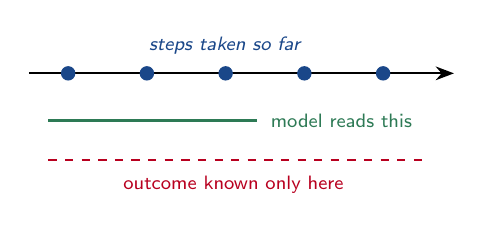
\begin{tikzpicture}[font=\scriptsize, >=Stealth]
  \draw[->, thick] (0,0) -- (5.4,0);
  \foreach \x in {0.5, 1.5, 2.5, 3.5, 4.5} \filldraw[accent] (\x,0) circle (2.4pt);
  \node[above, accent] at (2.5,0.12) {\textit{steps taken so far}};
  \draw[accent2, thick] (0.25,-0.6) -- (2.9,-0.6);
  \node[right, accent2] at (2.95,-0.6) {model reads this};
  \draw[warn, thick, dashed] (0.25,-1.1) -- (5.1,-1.1);
  \node[warn] at (2.6,-1.42) {outcome known only here};
\end{tikzpicture}
\end{center}
\begin{block}{The bar is not a coin flip}
\textbf{Counting the steps} already predicts the outcome --- the longer an
agent struggles, the likelier it fails. That trivial rule scores \g{58\,\%}.

\medskip
\bad{We have to beat 58\,\%, not 50\,\%.} Two independent checks put the floor
in the same place.
\end{block}
\end{column}
\end{columns}
\end{frame}

% ---------------------------------------------------------------- 2
\begin{frame}{Three findings}
\footnotesize
\begin{columns}[t]
\begin{column}{0.50\textwidth}
\textbf{1. A real gain, but uneven --- and pooling fixes the unevenness.}

\smallskip
Task families where the model beats step-counting:
\begin{center}\footnotesize
\begin{tabular}{lc}
\toprule
trained on coding tasks only & \bad{2 of 4} \\
trained on all task types    & \g{4 of 4}   \\
\bottomrule
\end{tabular}
\end{center}
\smallskip
The average hardly moves (67\,\% vs 58\,\%); the gain is that the answer stops
depending on which family you picked.

\medskip
\textbf{2. It does not survive a change of environment.}

\smallskip
Trained on software tasks, tested on household and desktop ones: \bad{49\,\%},
a coin flip, where counting steps gets 69\,\% --- and it stays confident while
wrong. Across families of the \emph{same} environment it works.
\end{column}
\begin{column}{0.48\textwidth}
\textbf{3. Rewarding the decision did not beat copying a teacher.}

\smallskip
Instead of matching a teacher's probability we rewarded the model for the
decisions its number caused: 71\,\% against 73\,\%. It works, but it is behind.

\medskip
\begin{block}{Where this leaves us}
Useful today as a cheap running estimate on coding agents --- quoted per task
family and against step-counting, never as one headline number.

\smallskip
Not yet a controller: it advises stopping 57\,\% of attempts where 60\,\%
would have succeeded.

\smallskip
The barrier is \emph{what the model reads}, not how it is trained.
\end{block}
\end{column}
\end{columns}
\end{frame}

\end{document}
